\FloatBarrier
\begin{appendices}
\chapter{Shared Memory for CUDA-Based Bitonic Sort}
\label{app:CUDABSShared}
\begin{figure}
\center
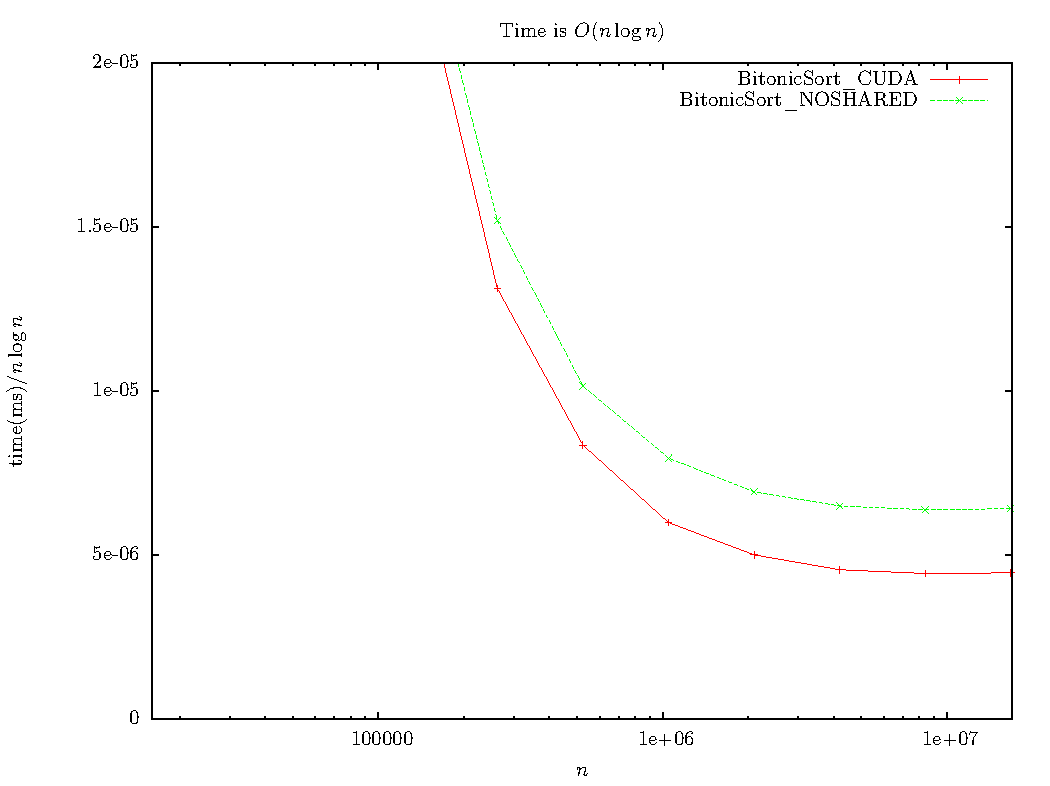
\includegraphics[width=\textwidth]{graphs/CUDAShared/nlogntime.pdf}
\caption{Running time of CUDA-based Bitonic Sort with and without shared memory, Quadro FX 880M}
\label{fig:CUDAShared}
\end{figure}
As mentioned in Section~\ref{sec:CUDAImpl}, utilizing shared memory for Bitonic Sort can be a big gain, and the graphs in the experiments section take advantage of this fact.
To further strengthen this claim, we have shown the effect of omitting the usage of shared memory in Figure~\ref{fig:CUDAShared}.

The figure clearly shows a major improvement in running time when utilizing shared memory.

\chapter{Fixed Sizes for Bitonic Sort}
\label{app:BitonicSize}
\begin{figure}
\center
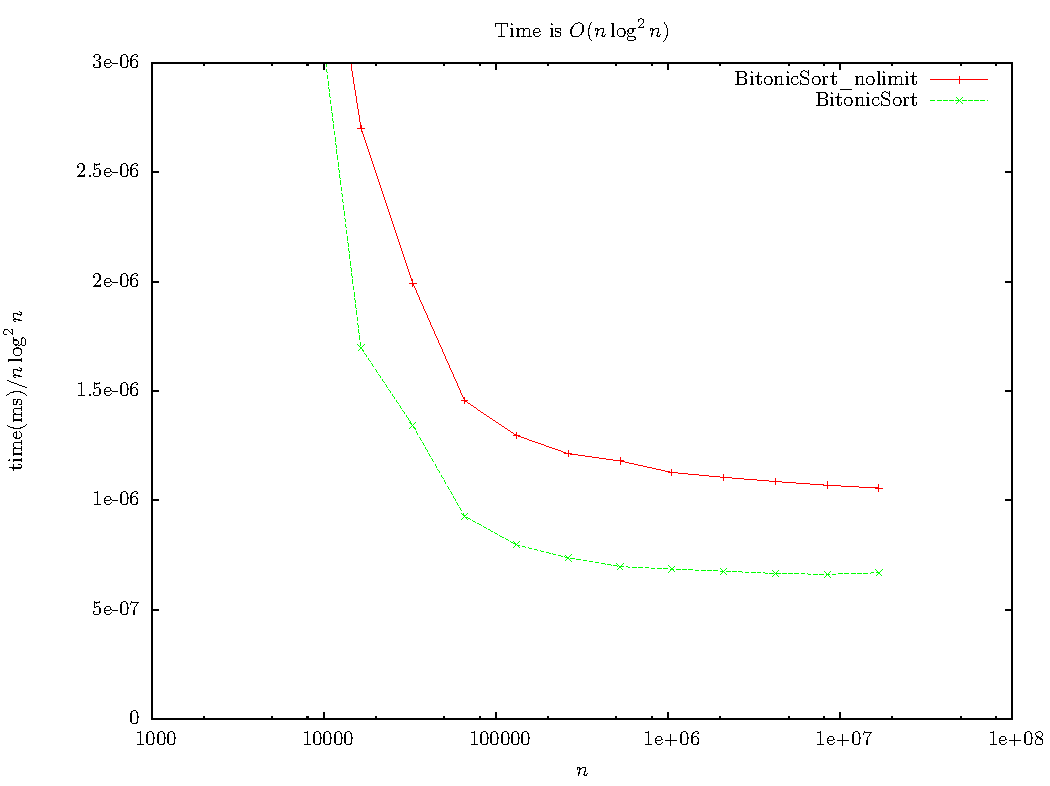
\includegraphics[width=\textwidth]{graphs/compiler/nlogntime.pdf}
\caption{Running time for Bitonic Sort, with and without fixed sizes}
\label{fig:BitonicSize}
\end{figure}
In Section~\ref{sec:BitonicImplementation} it is claimed that using fixed sizes for Bitonic Sort improves performance.

To support this claim, we have Figure~\ref{fig:BitonicSize}, that shows the optimized Bitonic sort in the experiments, compared to a version of Bitonic Sort that supports arbitrary input sizes, shown in the graph as \texttt{BitonicSort\_nolimit}.

\chapter{PRNG Effect on Performance}
\label{app:PRNG}
\begin{figure}
\center
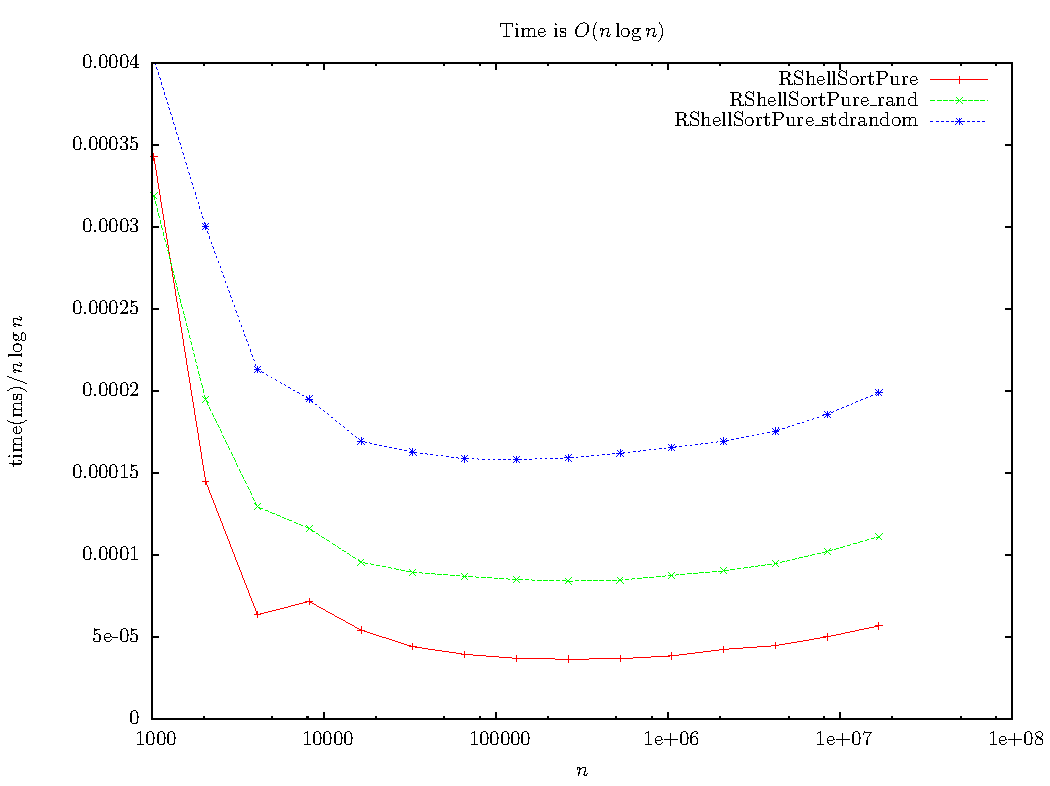
\includegraphics[width=\textwidth]{graphs/rand/nlogntime.pdf}
\caption{Running time for Randomized Shellsort, with varying PRNGs}
\label{fig:rand}
\end{figure}
Choosing a random number generator with good performance is very important for Randomized Shellsort, as noted in\ref{sec:PRNG}.

To show how big an effect the choice of PRNG actually has, which is shown in Figure~\ref{fig:rand}, where the optimized PRNG used in the experiments is compared to \texttt{rand} and \texttt{mt19937} from the \texttt{C++} standard library, shown in the graph as respectively as postfixes \texttt{\_rand} and \texttt{\_stdrandom}.
\end{appendices}
